
%% bare_jrnl_compsoc.tex
%% V1.4a
%% 2014/09/17
%% by Michael Shell
%% See:
%% http://www.michaelshell.org/
%% for current contact information.
%%
%% This is a skeleton file demonstrating the use of IEEEtran.cls
%% (requires IEEEtran.cls version 1.8a or later) with an IEEE
%% Computer Society journal paper.
%%
%% Support sites:
%% http://www.michaelshell.org/tex/ieeetran/
%% http://www.ctan.org/tex-archive/macros/latex/contrib/IEEEtran/
%% and
%% http://www.ieee.org/

%%*************************************************************************
%% Legal Notice:
%% This code is offered as-is without any warranty either expressed or
%% implied; without even the implied warranty of MERCHANTABILITY or
%% FITNESS FOR A PARTICULAR PURPOSE! 
%% User assumes all risk.
%% In no event shall IEEE or any contributor to this code be liable for
%% any damages or losses, including, but not limited to, incidental,
%% consequential, or any other damages, resulting from the use or misuse
%% of any information contained here.
%%
%% All comments are the opinions of their respective authors and are not
%% necessarily endorsed by the IEEE.
%%
%% This work is distributed under the LaTeX Project Public License (LPPL)
%% ( http://www.latex-project.org/ ) version 1.3, and may be freely used,
%% distributed and modified. A copy of the LPPL, version 1.3, is included
%% in the base LaTeX documentation of all distributions of LaTeX released
%% 2003/12/01 or later.
%% Retain all contribution notices and credits.
%% ** Modified files should be clearly indicated as such, including  **
%% ** renaming them and changing author support contact information. **
%%
%% File list of work: IEEEtran.cls, IEEEtran_HOWTO.pdf, bare_adv.tex,
%%                    bare_conf.tex, bare_jrnl.tex, bare_conf_compsoc.tex,
%%                    bare_jrnl_compsoc.tex, bare_jrnl_transmag.tex
%%*************************************************************************


% *** Authors should verify (and, if needed, correct) their LaTeX system  ***
% *** with the testflow diagnostic prior to trusting their LaTeX platform ***
% *** with production work. IEEE's font choices and paper sizes can       ***
% *** trigger bugs that do not appear when using other class files.       ***                          ***
% The testflow support page is at:
% http://www.michaelshell.org/tex/testflow/


\documentclass[10pt,conference,onecolumn,compsoc]{IEEEtran}


\usepackage{hyperref}
\usepackage{enumitem}
\setlist[itemize]{leftmargin=3 cm}
\setlist[enumerate]{leftmargin=3cm}



% *** CITATION PACKAGES ***
%
\ifCLASSOPTIONcompsoc
  % IEEE Computer Society needs nocompress option
  % requires cite.sty v4.0 or later (November 2003)
  \usepackage[nocompress]{cite}
\else
  % normal IEEE
  \usepackage{cite}
\fi
% cite.sty was written by Donald Arseneau
% V1.6 and later of IEEEtran pre-defines the format of the cite.sty package
% \cite{} output to follow that of IEEE. Loading the cite package will
% result in citation numbers being automatically sorted and properly
% "compressed/ranged". e.g., [1], [9], [2], [7], [5], [6] without using
% cite.sty will become [1], [2], [5]--[7], [9] using cite.sty. cite.sty's
% \cite will automatically add leading space, if needed. Use cite.sty's
% noadjust option (cite.sty V3.8 and later) if you want to turn this off
% such as if a citation ever needs to be enclosed in parenthesis.
% cite.sty is already installed on most LaTeX systems. Be sure and use
% version 5.0 (2009-03-20) and later if using hyperref.sty.
% The latest version can be obtained at:
% http://www.ctan.org/tex-archive/macros/latex/contrib/cite/
% The documentation is contained in the cite.sty file itself.



% *** GRAPHICS RELATED PACKAGES ***
%
\ifCLASSINFOpdf
   \usepackage[pdftex]{graphicx}
 
\else
 
\fi
% graphicx was written by David Carlisle and Sebastian Rahtz. It is
% required if you want graphics, photos, etc. graphicx.sty is already
% installed on most LaTeX systems. The latest version and documentation
% can be obtained at: 
% http://www.ctan.org/tex-archive/macros/latex/required/graphics/
% Another good source of documentation is "Using Imported Graphics in
% LaTeX2e" by Keith Reckdahl which can be found at:
% http://www.ctan.org/tex-archive/info/epslatex/
%
% latex, and pdflatex in dvi mode, support graphics in encapsulated
% postscript (.eps) format. pdflatex in pdf mode supports graphics
% in .pdf, .jpeg, .png and .mps (metapost) formats. Users should ensure
% that all non-photo figures use a vector format (.eps, .pdf, .mps) and
% not a bitmapped formats (.jpeg, .png). IEEE frowns on bitmapped formats
% which can result in "jaggedy"/blurry rendering of lines and letters as
% well as large increases in file sizes.
%
% You can find documentation about the pdfTeX application at:
% http://www.tug.org/applications/pdftex









% *** PDF, URL AND HYPERLINK PACKAGES ***
%
\usepackage{url}
% url.sty was written by Donald Arseneau. It provides better support for
% handling and breaking URLs. url.sty is already installed on most LaTeX
% systems. The latest version and documentation can be obtained at:
% http://www.ctan.org/tex-archive/macros/latex/contrib/url/
% Basically, \url{my_url_here}.




\begin{document}

\title{3ly-Zium\\ for UTM CSCI 352}
%
%

% received ..."  text while in non-compsoc journals this is reversed. Sigh.

\author{Colin Weatherly, Blade Johnson% <-this % stops a space
}

\IEEEtitleabstractindextext{%
\begin{abstract}
The project is a video game in the 2D platformer genre. The player is made to run through a level, and upon each successful completion, the level is changed to increase the difficulty. The intended target is people that play video games, primarily those that stream games as live reactions mesh well with high difficulties.
\end{abstract}

}


% make the title area
\maketitle



\IEEEdisplaynontitleabstractindextext

\IEEEpeerreviewmaketitle



\section{Introduction}



This project is a video game in the genre of 2D platformer. The goal of the game is to reach the exit of the level that the player character is placed in. The level’s layout will progressively get more complex with each clear, along with adding new hazards that increase the difficulty further. The penalty for failing a level is to be sent back to the beginning of said level, allowing the player to learn the level with every attempt.

The targeted audience for this project is people in the 18-34 age group who play video games on a regular basis. Specifically, those in the age group that livestream games. Due to the increasingly difficult challenge that the game provides, having live reactions of attempts to beat the game will provide content for the targeted audience.



\subsection{Background}
A 2D platformer is a game genre set on a 2D plane where the player controlled character must move and jump to avoid obstacles and reach the end.

We decided to make a platforming game because of our love for games in general and our shared interest in platformers. Because of this, we feel we can properly create one.

% needed in second column of first page if using \IEEEpubid
%\IEEEpubidadjcol


\subsection{Impacts}
This project is not meant to impact the world in some way. The point of a game is to provide entertainment, which will only impact a portion of the population if it were to gain traction within the community. At the current time, there is no plan for a meaningful story in the game, so the impact will be purely driven by the quality of the gameplay.

\subsection{Challenges}
The main challenges will most likely be coding the physics of the player character; developing new mechanics instead of being purely moving and jumping; keeping the game fun despite the difficulty.


\section{Scope}
This platforming game is considered done once three levels of the game are playable from start to finish with minimal bugs or exploits. The player should be able to get through these stages without too much unnecessary frustration with either the difficulty of these stages or the control of the player character. The player character should be fully implemented with all moves intact (moving, jumping) and all hazards(such as spikes) should fail the level upon contact with the player character. As a stretch goal, we want to include more levels with new hazards. An additional stretch goal is the addition of extra moves(i.e walljumping, sliding) the player character requires to progress in more difficult levels. An additional stretch goal is scaling the window and the game assets to fit more than one resolution.

\subsection{Requirements}

\subsubsection{Functional}
\begin{itemize}
\item Player's completed levels stay completed – user's completed levels persist after the application is exited and started again
\item User inputs via designated keys are read – the application should register the inputs and move the player character accordingly
\item Selecting New Game erases the user's save data – completed levels will return to being uncompleted, player is loaded into the first level as if starting the game for the first time
\item Level fails upon contact with a hazard – should the player character run into a hazard(i.e spike), level is failed and character is returned to the starting point of the same level
\end{itemize}

\subsubsection{Non-Functional}
\begin{itemize}
\item The game correctly displays in a 1280x720 resolution window
\item The game runs at a smooth framerate, preferably 30 frames per second
\item User's inputs have little to no delay, preferably under half a second
\end{itemize}

\subsection{Use Cases}
These are cases in which the user will interact with the program's user interface. The use cases can be seen in Table \ref{tab:useCaseIndex}.




\begin{table}
\centering
\begin{tabular}{|c|c|c|c|c|}
\hline
Use Case ID & Use Case Name & Primary Actor & Complexity & Priority \\
\hline \hline
1 & Start New Game & User & Low & 1\\
\hline
2 & Level Select & User & Low & 1\\
\hline
3 & Character Jump & User & Medium & 1\\
\hline

\end{tabular}
\caption{Use case table}
\label{tab:useCaseIndex}
\end{table}


\begin{itemize}
\item[Use Case Number:] 1
\item[Use Case Name:] Start New Game
\item[Description:] The player decides to begin the game from the beginning (Level 1). They will click on the ``New Game" button (see Figure \ref{Start Mockup}). This will load the first level of the game (see Figure \ref{Level Mockup}). NOTE:This is only a conceptualized level meant to show loading into a level, not specifically level 1.
\end{itemize}

Process flow:

\begin{enumerate}
\item Player starts the program, which begins with the main menu loaded.
\item The player left-clicks the ``New Game" option on the menu.
\item The game state is updated to gameplay, and the first level is loaded.
\item[Termination Outcome:] Gameplay has begun in level 1.
\end{enumerate}

\begin{itemize}
\item[Use Case Number:] 2
\item[Use Case Name:] Level Select
\item[Description:] The player is on the main menu. The player wishes to choose a specific level in the game to play. They will left-click the ``Level Select" button on the main menu, and the screen will update to show a list of levels in vertical descending order. The player then left-click a button corresponding to a specific level, and the game will load the corresponding level (see Figure \ref{Select Mockup}).
\end{itemize}

Process flow:

\begin{enumerate}
\item Player starts the program, which begins with the main menu loaded.
\item The player left-clicks the ``Level Select" option on the main menu.
\item The level select screen is loaded, showing each level vertically in numerically descending order.
\item The player left-clicks the option corresponding to their desired level.
\item The game state is updated to gameplay, and the corresponding level loads.
\item[Termination Outcome:] Gameplay has begun in the player's selected level.
\end{enumerate}

\begin{itemize}
\item[Use Case Number:] 3
\item[Use Case Name:] Character Jump
\item[Description:] The player is in gameplay. They wish to make the player character jump (in order to avoid hazards such as spikes). The player then hits the space bar. The player character will then leap upward. The character will gradually rise up off the ground for a few seconds, then gradually fall back to the ground.
\end{itemize}

Process flow:

\begin{enumerate}
\item Player is in a stage of gameplay.
\item The player presses the space bar.
\item The player character then leaps off the ground into the air.
\item After a few seconds of gradually rising upward, the player character then gradually falls until hitting the ground.
\item[Termination Outcome:] The player character has completed a full jump.
\end{enumerate}

Alternative: Player character is already jumping
\begin{enumerate}
\item The player presses the space bar as the player character is in mid-jump.
\item The player character performs a rotation mid-jump.
\item Outcome is dependent on whether the player contacts a wall.
\item[Termination Outcome:] If the player contacts a wall they will be launched away from the wall horizontally. Else, the player will complete a full jump as if they had inputted a normal jump.
\end{enumerate}


\subsection{Interface Mockups}
\begin{figure}[ht!]
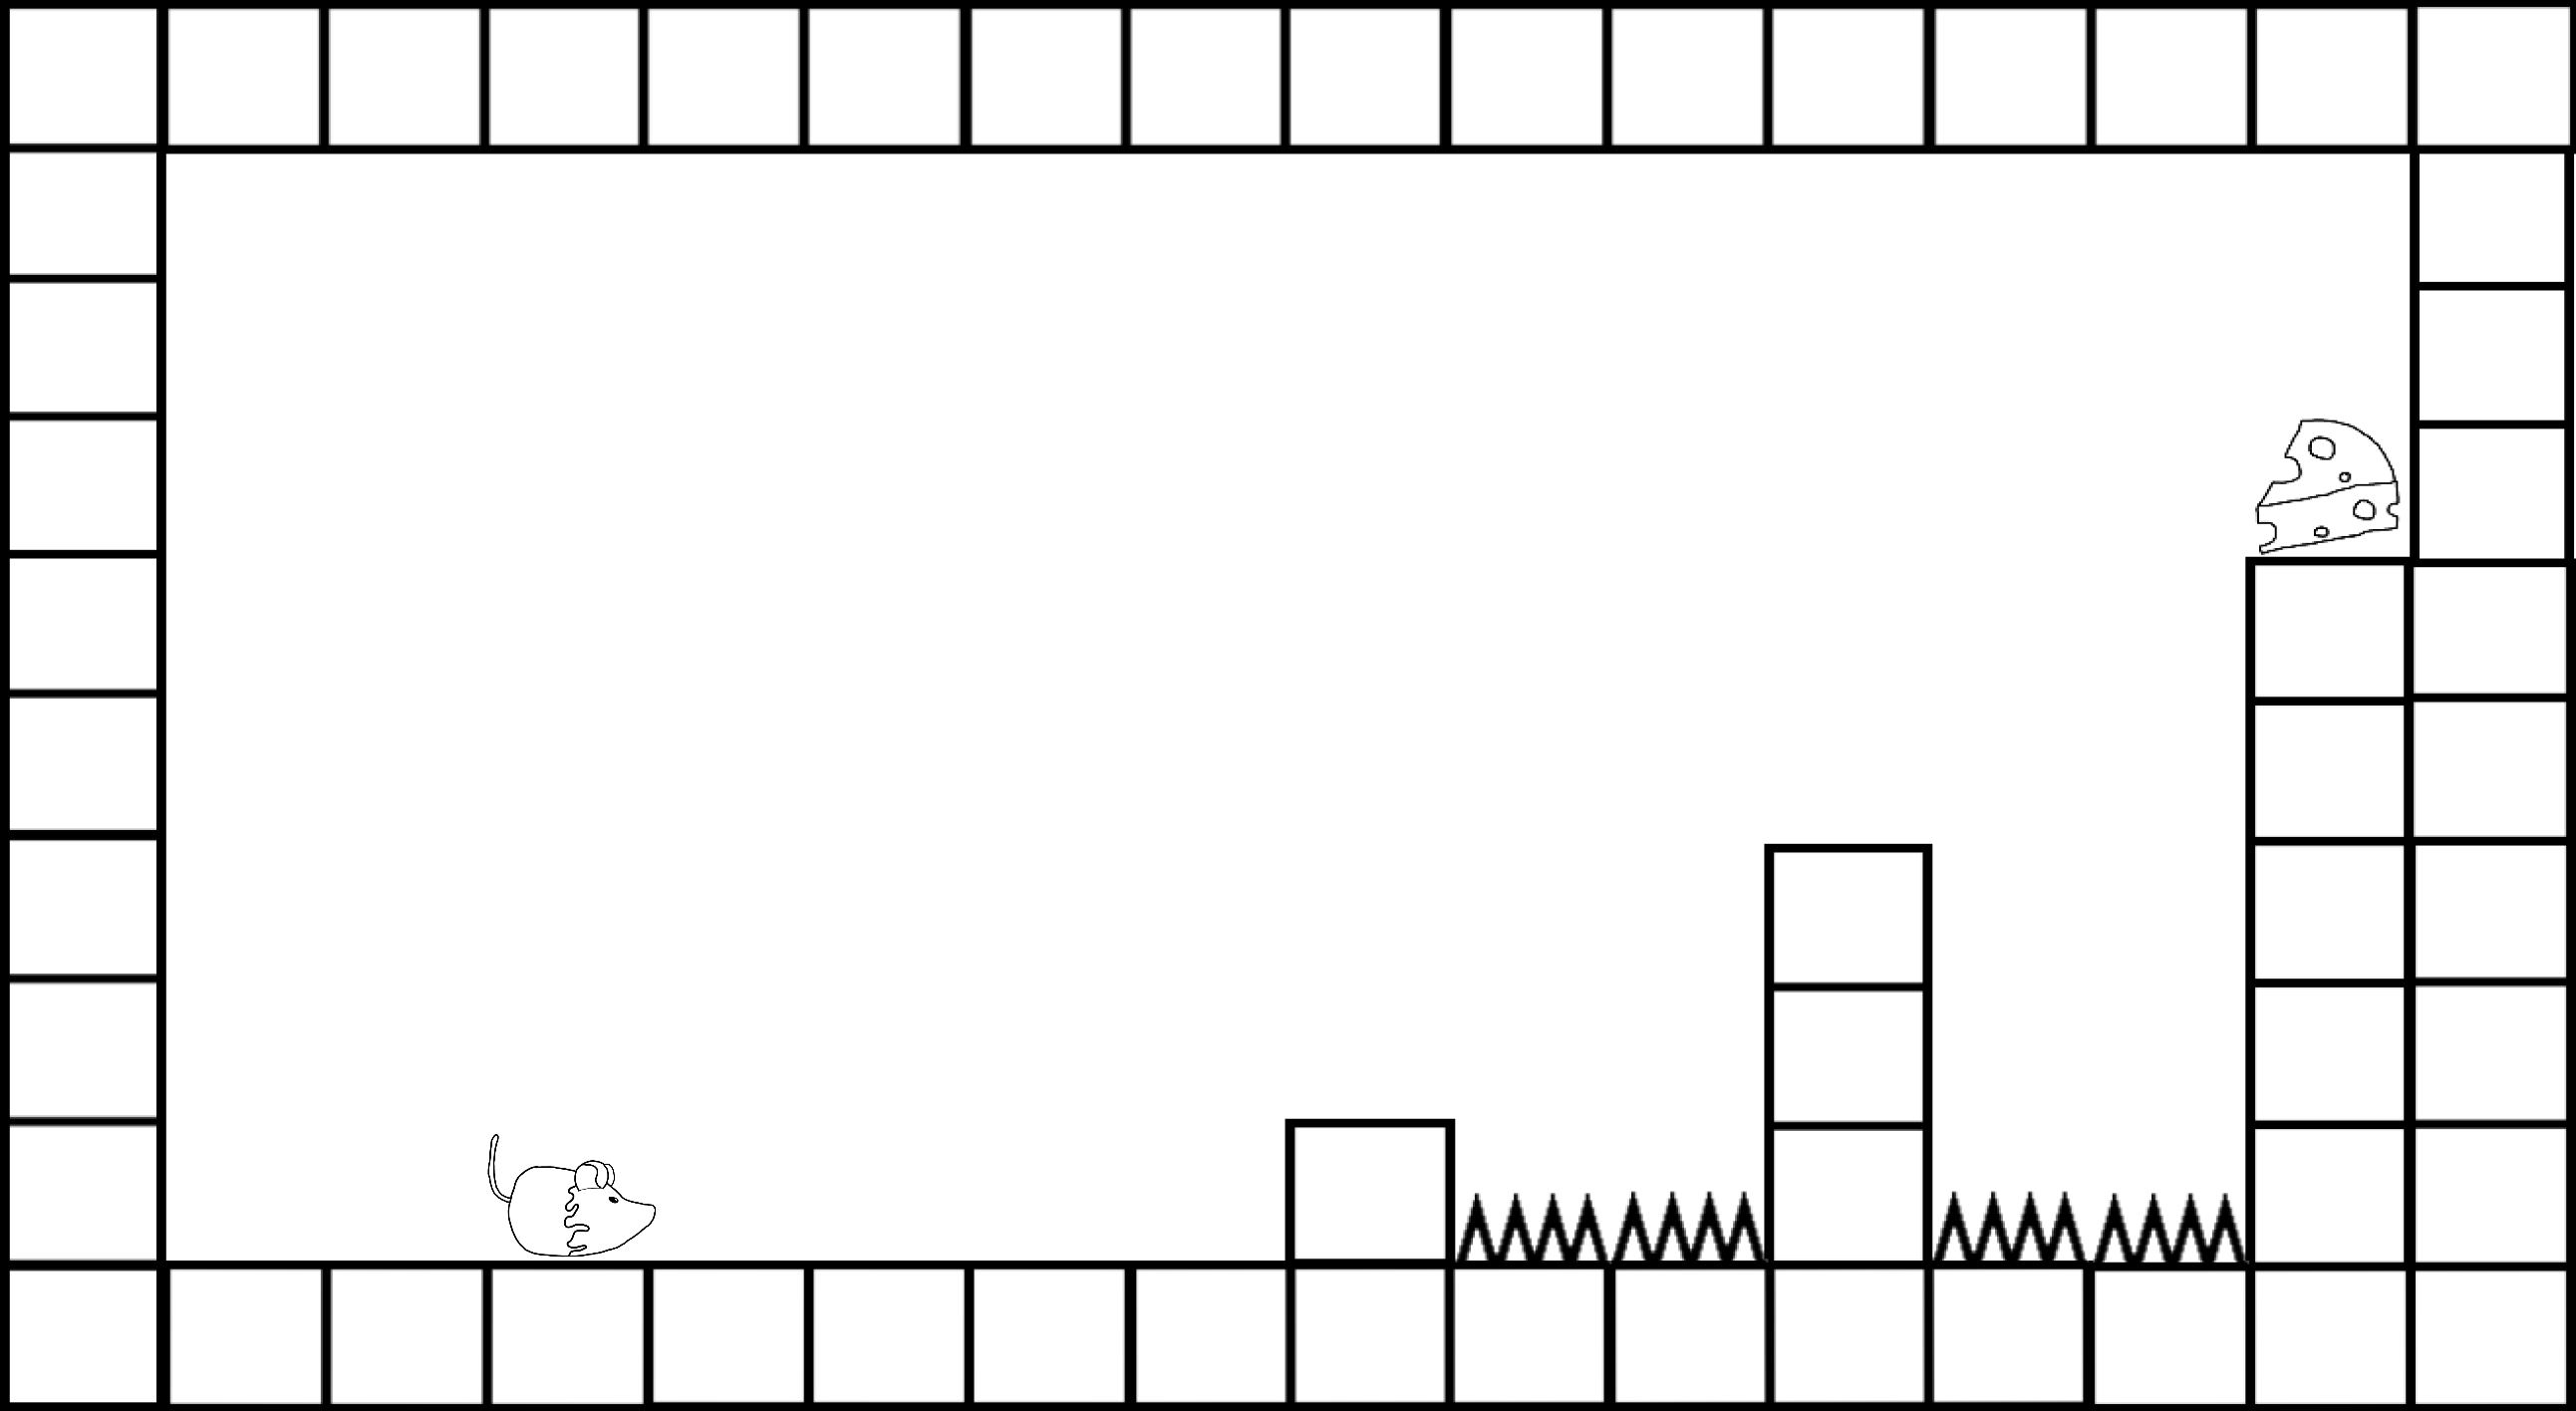
\includegraphics[height=250px, width=400px]{Level Mockup.png}
\caption{Mockup of a player loading into a level}
\label{Level Mockup}
\end{figure}

\begin{figure}[ht!]
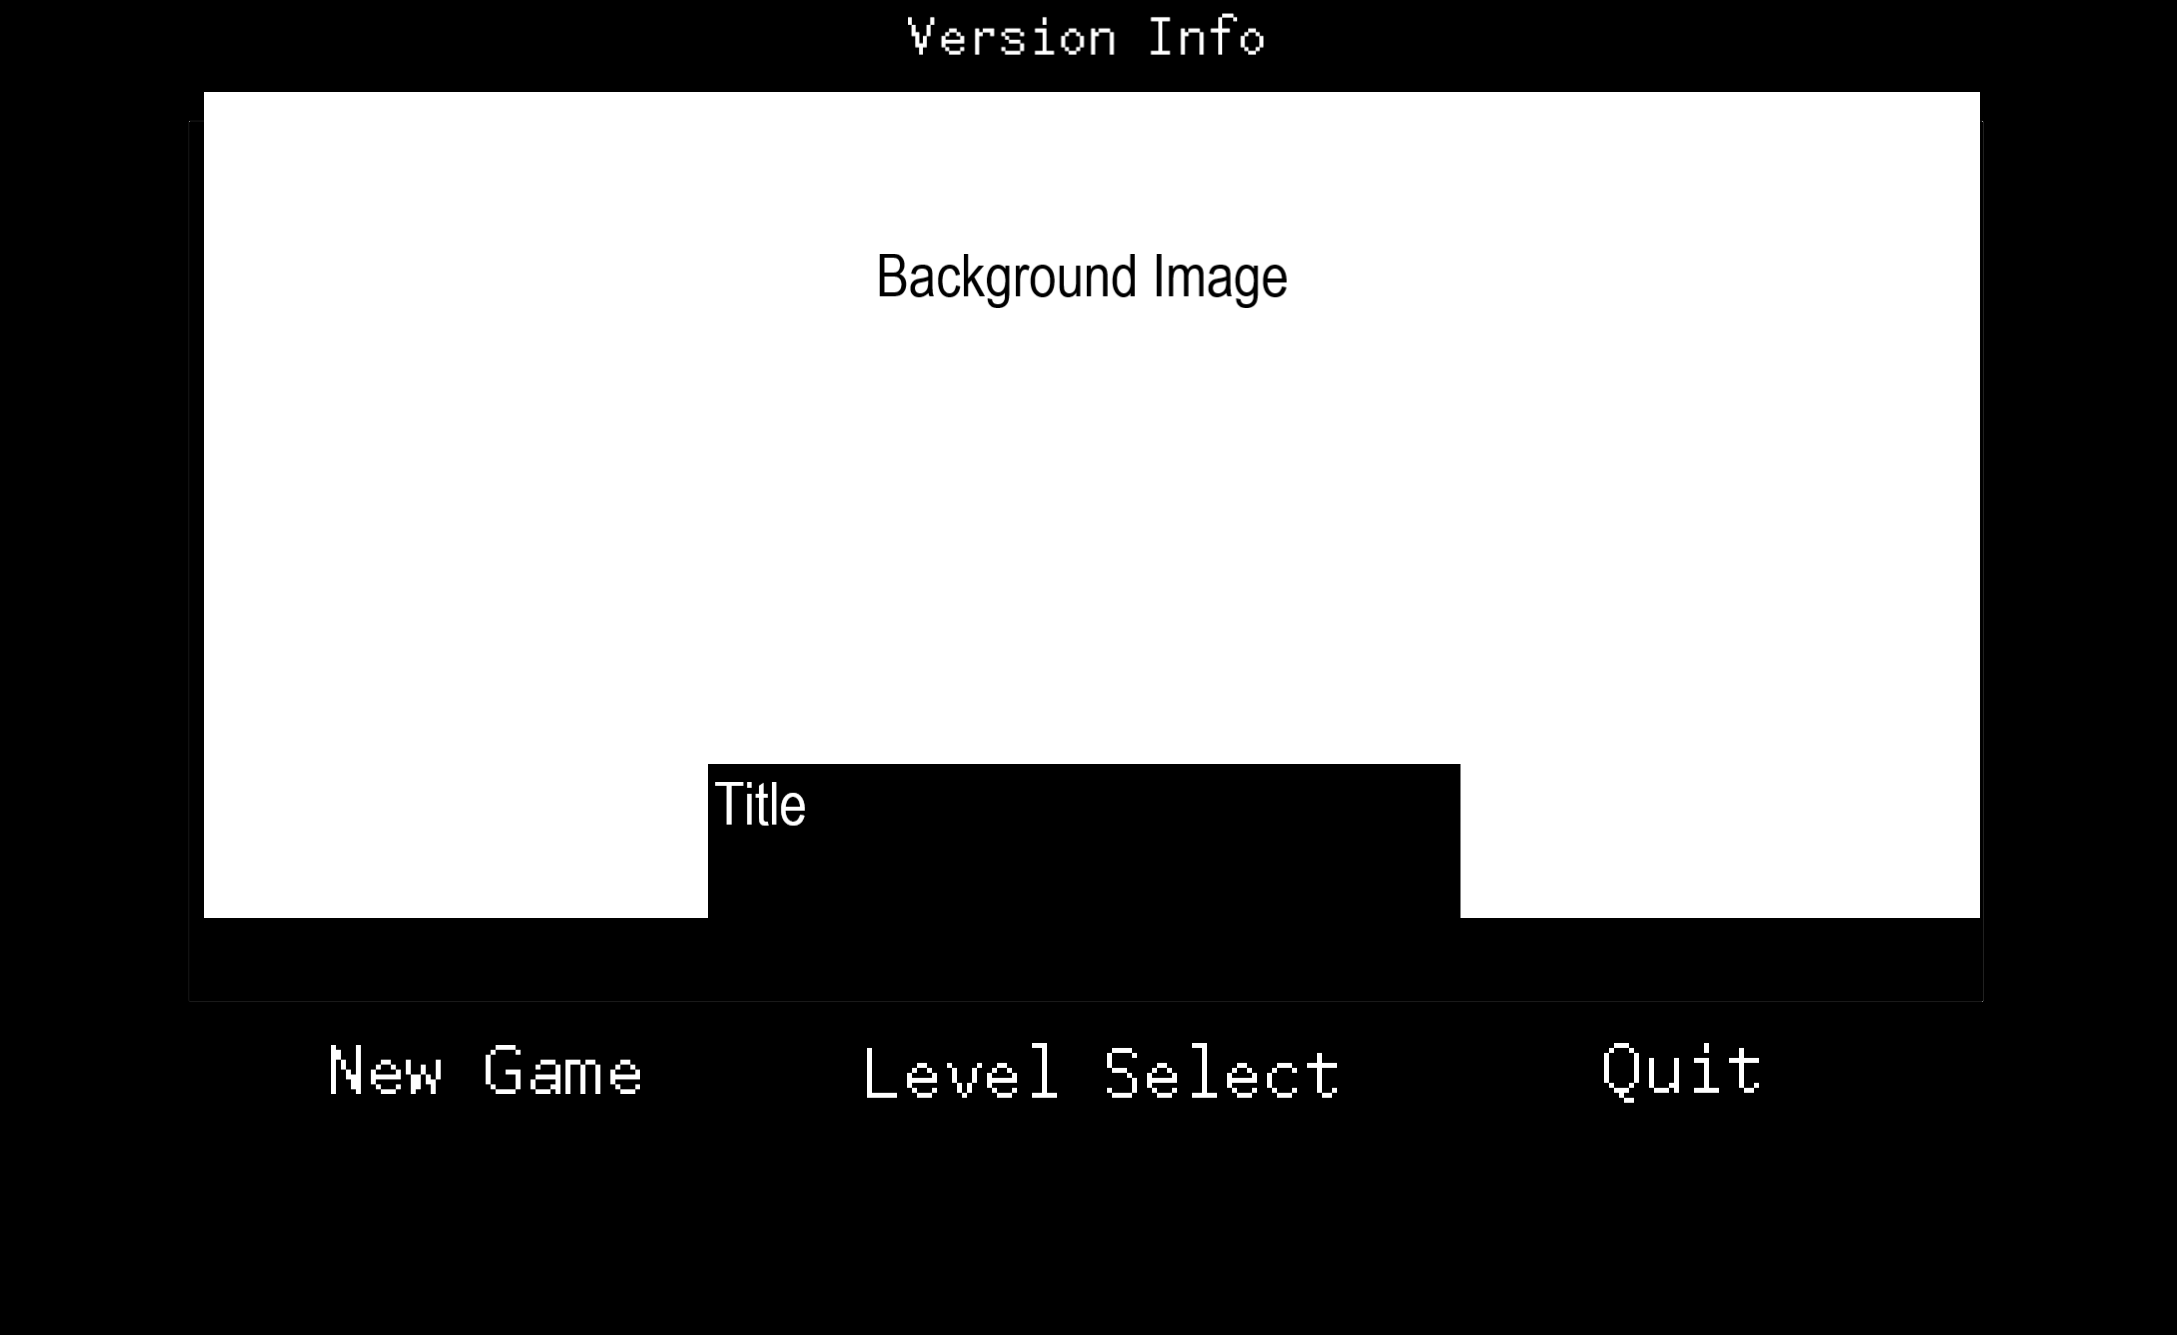
\includegraphics[height=250px, width=400px]{Start Mockup.png}
\caption{Mockup of the main menu screen}
\label{Start Mockup}
\end{figure}

\begin{figure}[ht!]
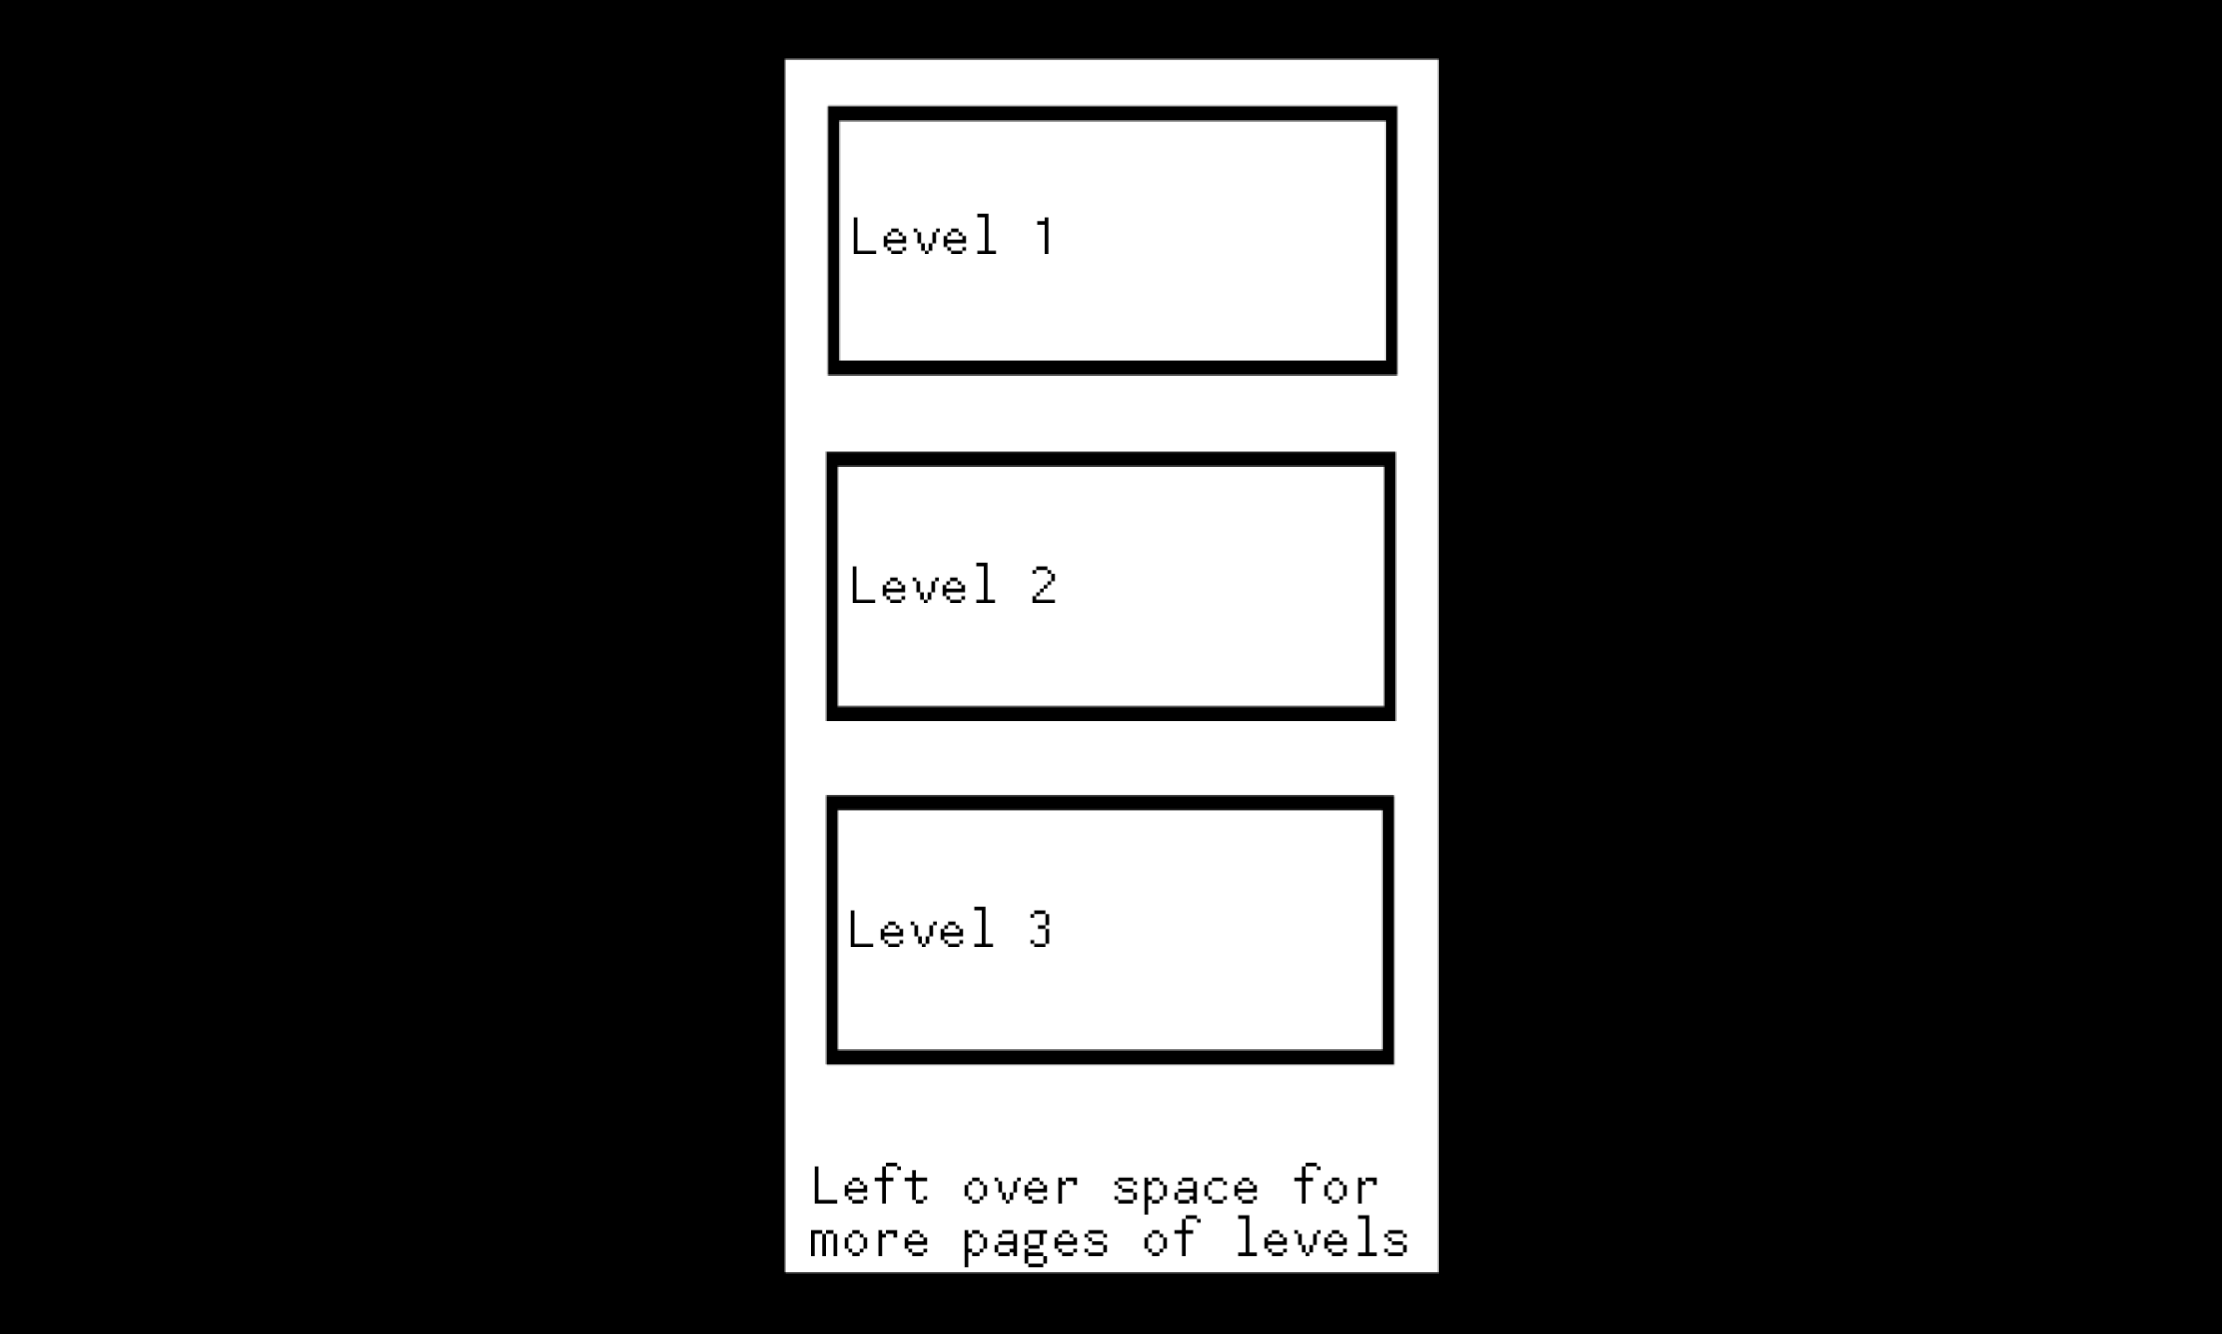
\includegraphics[height=250px, width=400px]{Select Mockup.png}
\caption{Mockup of the level select screen}
\label{Select Mockup}
\end{figure}



\section{Project Timeline}
Refer to Figure \ref{Timeline}.
\begin{figure}[ht!]
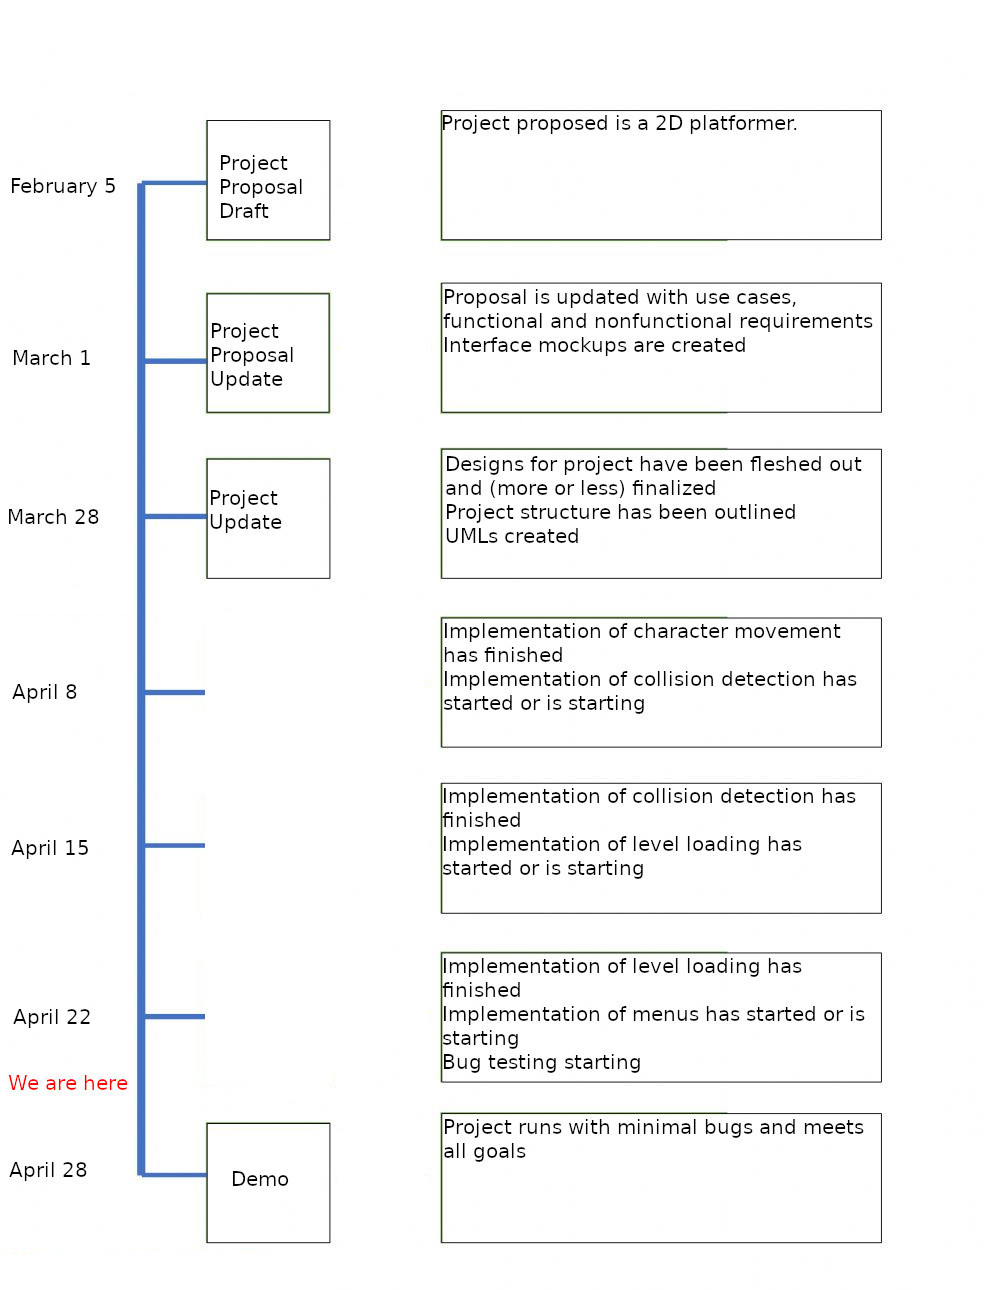
\includegraphics[height=400px, width=300px]{Timeline.jpg}
\caption{Timeline}
\label{Timeline}
\end{figure}


\section{Project Structure}
At first, this will be a little empty (it will need to be filled in by the time you turn in your final report).  This is your chance to discuss all of your design decisions (consider this the README's big brother).

\subsection{UML Outline}
Facade: refer to Figure \ref{Facade}.
\begin{figure}[ht!]
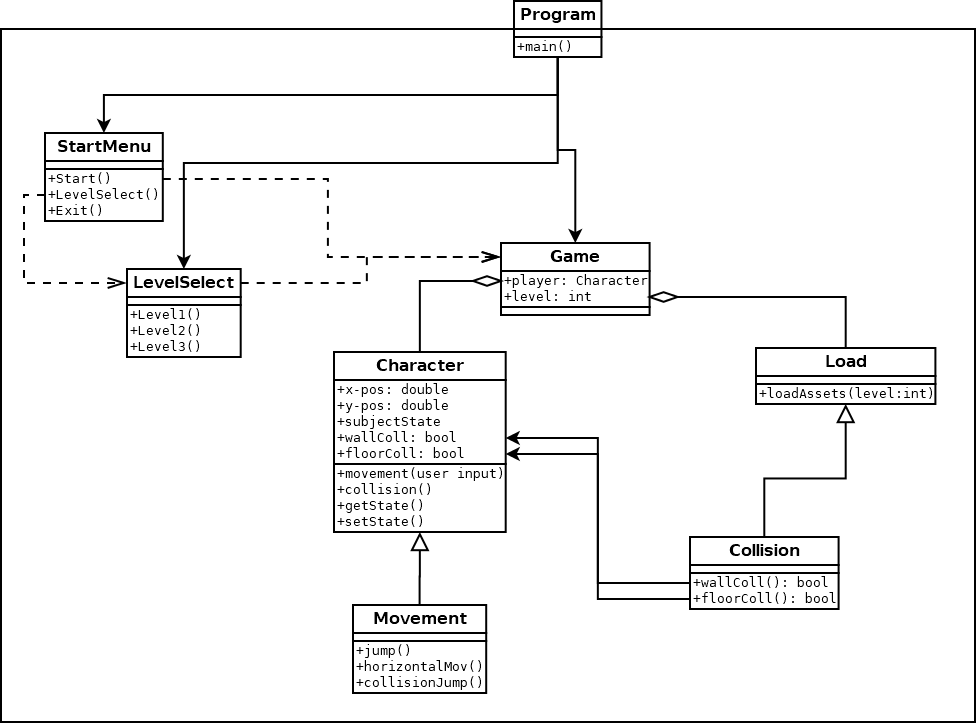
\includegraphics[height=350px, width=400px]{Facade.png}
\caption{Facade Outline}
\label{Facade}
\end{figure}

\begin{figure}[ht!]
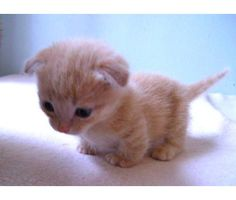
\includegraphics[scale=1.5]{cat2.jpg}
\caption{Morale Support}
\label{cat2}
\end{figure}


\subsection{Design Patterns Used}
Make sure to actually use at least 2 design patterns from this class.  This is not normally part of such documentation, but largely just specific to this class -- I want to see you use the patterns!


\section{Results}
This section will start out a little vague, but it should grow as your project evolves.  With each deliverable you hand in, give me a final summary of where your project stands.  By the end, this should be a reflective section discussing how many of your original goals you managed to attain/how many desired use cases you implemented/how many extra features you added.

\subsection{Future Work}
Where are you going next with your project?
For early deliverables, what are your next steps?  (HINT: you will typically want to look back at your timeline and evaluate: did you meet your expected goals?  Are you ahead of schedule?  Did you decide to shift gears and implement a new feature?)
By the end, what do you plan on doing with this project?  Will you try to sell it?  Set it on fire?  Link to it on your resume and forget it exists?




\begin{thebibliography}{1}

\bibitem{IEEEhowto:kopka}
H.~Kopka and P.~W. Daly, \emph{A Guide to \LaTeX}, 3rd~ed.\hskip 1em plus
  0.5em minus 0.4em\relax Harlow, England: Addison-Wesley, 1999.

\end{thebibliography}



\begin{IEEEbiography}{Michael Shell}
Biography text here.
\end{IEEEbiography}

% if you will not have a photo at all:
\begin{IEEEbiographynophoto}{John Doe}
Biography text here.
\end{IEEEbiographynophoto}

% insert where needed to balance the two columns on the last page with
% biographies
%\newpage

\begin{IEEEbiographynophoto}{Jane Doe}
Biography text here.
\end{IEEEbiographynophoto}





% that's all folks
\end{document}


